\section{Постановка задачи}

\begin{enumerate}
\item Построить график $N$ первых членов логистического отображения, предусмотреть возможность изменения параметров отображения;
\item Построить бифуркационную диаграмму отдельными точками и непрерывной линией, определить положение точек бифуркации;
\item Исследовать полученные графики.
\end{enumerate}

\section{Математическая модель}

Логистическое отображение задается рекуррентным соотношением
%%
\begin{equation}
x_{n+1} = R x_n \left(1 - x_n\right) \textrm{,}
\end{equation}
%%
где $R$ -- некоторый параметр. Можно показать, что данный ряд сходится к некоторому $x_k \in \left[0..1\right]$ при $x_0 \in \left[0..1\right]$ и $R \in \left[0..4\right]$.

Бифуркационная диаграмма являет собой зависимость некоторого $k$-го члена ряда от $R$. Вся диаграмма может быть получена многократным построением $x_k(R)$ с разными $x_0$.

Логистическое отображение используется в частности для демонстрации и изучения хаотических систем, т.е. систем, для которых минимальные изменения в начальных условиях вызывают значительное изменение поведения.

\section{Численная модель}

В то время как вычисление $x(n)$ является довольно тривиальной задачей, построение бифуркационной диаграммы сопряжено с некоторыми трудностями.

Для построения точечной бифуркационной диаграммы для каждого $R_i = R_0 + i\varepsilon$ в диапазоне изменения $R$ вычислялось некоторое количество $x_k$ с разными (случайными) $x_0$.

Соединение точек диаграммы производилось по критерию минимальности Евклидового расстояния между точками с $R = R_{i}$ и $R = R_{i - 1}$ (точка множества $\left\{R = R_{i}\right\}$ соединялась с той точкой множества $\left\{R = R_{i - 1}\right\}$, расстояние до которой минимально).

\section{Результаты и их обсуждение}

В ходе работы была написана демонстрационная программа на языке $c++$. Программа позволяет исследовать зависимость $x(n)$ для нескольких первых членов ряда при разных начальных параметрах и зависимость $x_k(R)$ при различном номере члена $k$. Программа также находит и отображает первые несколько точек бифуркации и их координаты.

Внешний вид программы приведен на \autoref{fig:mainwindow}.

\begin{figure}[h]%
\centering
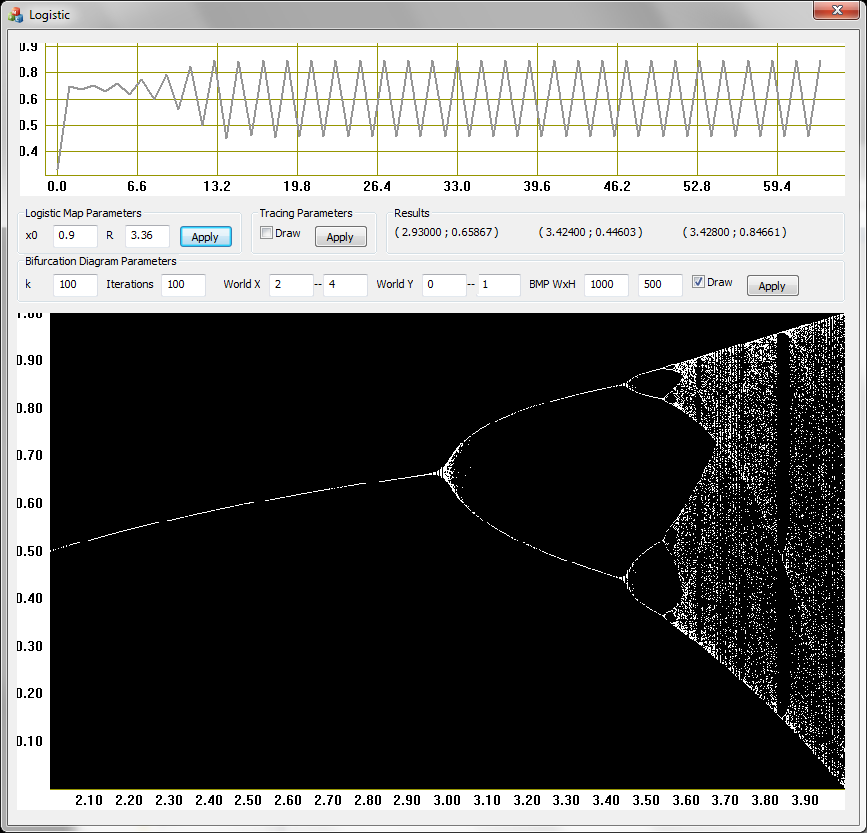
\includegraphics[width=0.6\textwidth]{mainwindow}%
\caption[Главное окно программы.]{Главное окно программы}%
\label{fig:mainwindow}%
\end{figure}

Можно видеть, что до точки $R \approx 2.998$ график $x_k(R)$ имеет одну ветку. После чего веток становится две. При $R \approx 3.448$ каждая ветка разделяется еще на две. После нескольких дальнейших бифуркаций график приобретает хаотическое поведение.

\begin{figure}[h]%
\centering
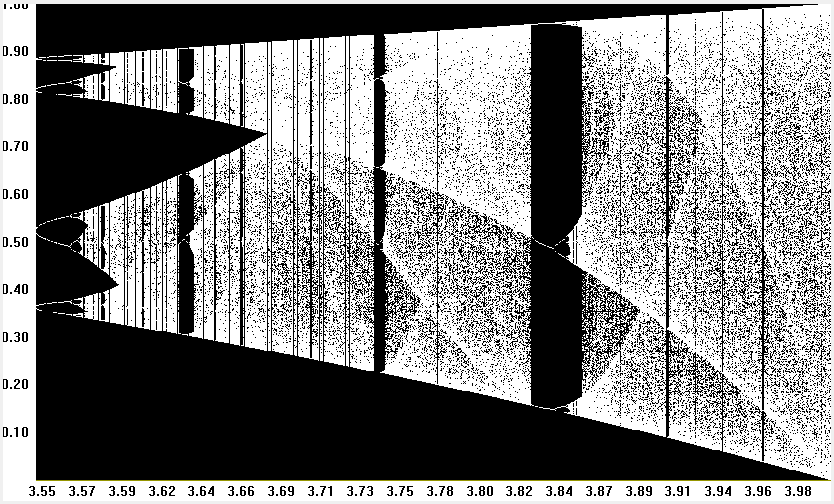
\includegraphics[width=0.6\textwidth]{right_area}%
\caption[Правая половина графика.]{Правая половина графика}%
\label{fig:right_area}%
\end{figure}

На \autoref{fig:right_area} показана увеличенная правая часть бифуркационной диаграммы (начиная с $R \approx 3.5$). Здесь ясно видны вертикально ориентированные области, в которых, по сравнению с окружающим пространством, очень малая концентрация точек. На \autoref{fig:gap} показана одна из таких областей. В ней обнаруживаются те же структуры, что и в начальной (левой) области диаграммы (при $R \lesssim 3.5$). Можно сказать, что диаграмма является \enquote{самоподобной}.

\begin{figure}[h]%
\centering
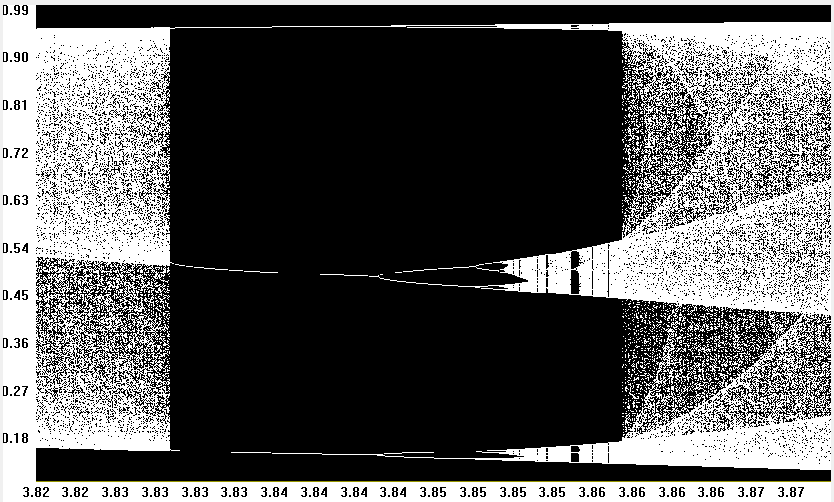
\includegraphics[width=0.6\textwidth]{gap}%
\caption[Область с малой концентрацией точек.]{Область с малой концентрацией точек}%
\label{fig:gap}%
\end{figure}

\section{Выводы}

В ходе работы была написана демонстрационная программа для исследования поведения хаотической системы -- логистического отображения.

Был проанализирован внешний вид бифуркационной диаграммы отображения, определены некоторые ее параметры.

Выяснилось, что диаграмма является \enquote{самоподобной}, т.е. содержит однотипные структуры, по внешнему виду напоминающие графическое представление бинарного дерева.

Были определены координаты первых трех точек бифуркации: $P_1 = \left(2.998, 0.66644\right)$, $P_{21} = \left(3.448, 0.44031\right)$, $P_{22} = \left(3.448, 0.84971\right)$ (дискретность шага по $R$ -- $0.002$).